The growing importance of cryptocurrency in a global market where facing a potential economic crisis in which fiat money might not be anymore the common exchange medium between different parties. The technological development and amazing availability of growing data to explore are the key factors that led to research on cryptocurrency and try to analyze through machine learning and distributed systems the potential price fluctuations. 
Another point to consider: Social media plays nowadays an important role in our daily life, more and more politicians use these platforms for instant communications, researchers announce publications and press uses them as a main platform to publish breaking news. All in all, we cannot take out anymore social media from the impact of our economic and political situations. It is therefore important to consider this as a key factor in the market decisions made on daily basis and the price fluctuations of the assets.

The main idea is to use a big cryptocurrency data set and a trained model of cryptocurrency related news to predict short term future prices for all the provided asset by using Machine learning algorithms. 

\subsection{Cryptocurrency}

Cryptocurrency can be defined as “a digital asset designed to work as a medium of exchange that uses strong cryptography to secure financial transactions, control the creation of additional units, and verify the transfer of assets.” \cite{noauthor_what_2020} Cryptocurrencies use decentralized control as opposed to centralized digital currency and central banking systems, which means no central entity has full control or power over the asset, but the community maintains it through systems known as “nodes” and each transaction is recorded in a public ledger known as the “blockchain”\footnote{A blockchain is a time-stamped series of immutable records of data that is managed by a cluster of computers not owned by any single entity. Each of these blocks of data (i.e. block) is secured and bound to each other using cryptographic principles (i.e. chain). public to anyone and resilient to changes. It is therefore virtually impossible to commit fraud if more than 50\% of the computational resources belong to the community and not the entity intending to hack or modify the blockchain\cite{ameer_rosic_what_2016}}

\subsubsection{Cryptocurrency Data set}

The data set used for this project is a Binance exchange data set extracted from the portal Kaggle\cite{smit_binance_2020}. The data set is titled “Binance Full History” and contains 1 minute candlestick data for a total of 786 cryptocurrency pairs traded on the exchange Web portal Binance.com\cite{binance_bitcoin_2020}. 
The features of this data set are:
\begin{itemize}
    \item Data types: python-pandas parquet files\footnote{pandas is a Python package providing fast, flexible, and expressive data structures designed to make working with "relational" or "labeled" data both easy and intuitive. It aims to be the fundamental high-level building block for doing practical, real world data analysis in Python \cite{noauthor_pandas_2020}. Parquet files are compressed binary files specially built to reduce storage size of big data files and improve loading performance.}
    \item Data size : 10GB
    \item Number of files : 764
\end{itemize}

\begin{figure}[H]
   \centering
   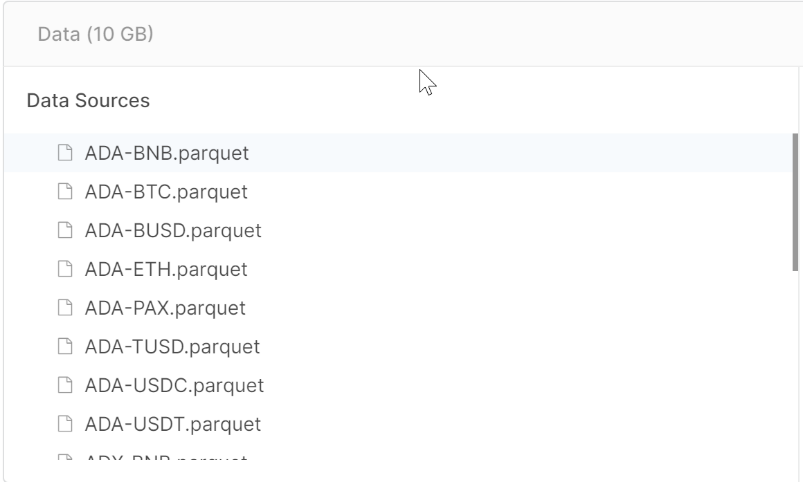
\includegraphics[width=\linewidth]{fig/CryptocurrencyDataSetParquetFiles.png}
    \caption{Cryptocurrency data set. Parquet file (taken from \cite{smit_binance_2020})}
    \label{fig:CryptoCurrencyDatasetParquet}
\end{figure}

\subsubsection{Cryptocurrency data set features and details}

A minute candlestick represents the maximum and minimum price at which any given asset was sold. It also contains information about the open price (price at the beginning of the time) and close price (end of time). 

\begin{figure}[h]
   \centering
   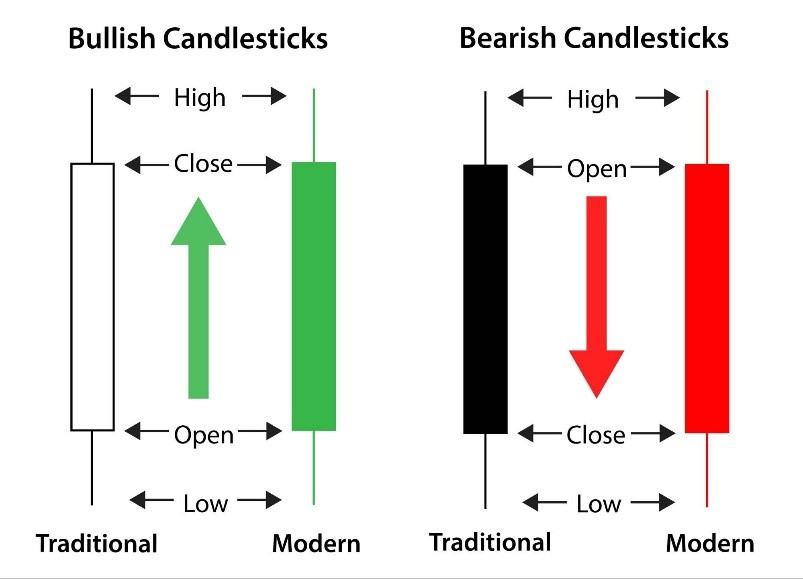
\includegraphics[width=\linewidth]{fig/CandlestickRepresentation.jpg}
    \caption{Candlestick Representations}
    \label{fig:CryptoCurrencyDatasetParquet}
\end{figure}

A series of candlestick represent the market fluctuation in a given period of time. 

\subsection{News data set}

The news data set was extracted from the web portal “CoinTelegraph.com”\footnote{The most recent news about crypto industry at Cointelegraph. Latest news about bitcoin, ethereum, blockchain, mining, cryptocurrency prices and more\cite{cointelegraph_cointelegraph_2013}} .
The data set was created using python scripts due to the lack of availability of a full set. 

The features of this data set are:

\begin{itemize}
    \item Data types: 2 \csv files total size is 128 MB.
    \item More than 20,000 different news from 2013 until present for human-written news about cryptocurrency and related subjects.
    \item Header file. Contains relevant metadata information about the news (such as title, thumbnail, creation date, etc.).
    \item Content file. Contains the body of the news and other metadata like the number of views and times it has been shared as well as image references for it.
\end{itemize}

\begin{figure}[h]
   \centering
   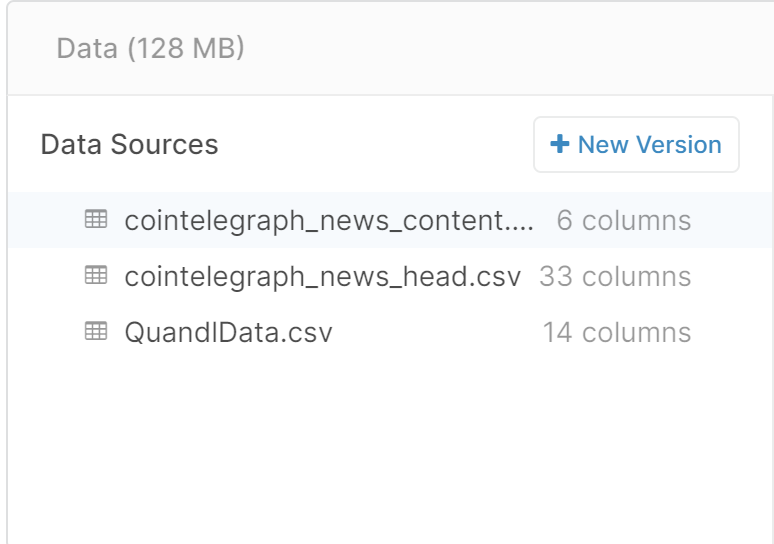
\includegraphics[width=\linewidth]{fig/CryptocurrencyNewsDataSet.png}
    \caption{Cryptocurrency News Data set \cite{cantu_cryptocurency_2020}}
    \label{fig:CryptoCurrencyNewsDataset}
\end{figure}


\subsection{Related works}
Several attempts and previous works from the data science community have been made to predict stock market price using Machine learning. The procedures and models are not so much different from the cryptocurrency model since both are time series models and its current input depend directly on past data. There is, however one big difference: the price volatility, which leads to the research no model training and adjustment to compensate for the possible increases and at the same time adapt the model to avoid overfitting.

For this project and among other sources three jobs were considered as role models:

\citeauthor{xavier_predicting_2019} approaches in his research document different Machine Learning models and mechanisms to predict tock market prices by performing Moving Average and LSTM\footnote{Acronymm for Long Short-Term Neural network. A special kind of Neuran network model that is trained based on past data.} training models. His results show the differences in the accuracy for the two different models and make evident that LSTM model performs better, although several adjustments have to be done depending on the asset to model.  \cite{adusumilli_predicting_2020} 

\citeauthor{pablo_castilla_predict_2018} takes the theory of LSTM into practice in a kaggle document, and figures the basic mecanishm for data processing, normalization and training\cite{pablo_castilla_predict_2018}.

Finally the work from \citeauthor{sagar_cryptocurrency_2019} addresses the machine learning mechanisms for cryptocurrency trading. Part of his research is used to tune and develop the Machine learning algorithms.





